Mezní kmitočet navrhovaného filtru byl zvolen v řádu stovek kHz, což umožňuje využití např. pro přenos rozhlasového vysílání v atmosféře, nebo monitorování EKG přenosným zařízením (Shueen-Yuh, Chih-Jen \cite{1}). \\ 
\\
Kmitočet v řádu stovek kHz odpovídá dlouhým a středním vlnám. Dlouhé vlny (30--300~kHz, čemuž odpovídá délka vlny 1--10~km) obtékají nerovnosti a jdou za obzor bez nutnosti odrazu. Dnes na dlouhých vlnách vysílá jen několik národních rozhlasových vysílačů velkých států a pásmo se hlavně využívá pro takové účely, kde je na prvním místě spolehlivost a výhody pozemní vlny. To jsou například frekvenční a časové standardy (DCF77 - rádiová stanice vysílající dlouhovlnný tzv. frankfurtský časový signál), radiomajáky, případně i komunikace s ponorkami \cite{2}. \\
\\
Střední vlny (525--1705~kHz, což odpovídá vlnovým délkám 186--577 m) mají menší dosah a často u nich dochází k jednomu odrazu od atmosféry. Lépe se ohýbají za přírodními překážkami a jsou vhodné pro vysílání v okruhu stovek kilometrů \cite{3}. \\
Po zvýšení mezního kmitočtu, aby odpovídal standardu ZigBee, možné využití ve WSN (\textit{Wireless Sensor Network}) pro monitorování dat z environmentálních senzorů v dané lokalitě. WSN běžně používá standard ZigBee s frekvencemi 868~MHz, 902–928~MHz a 2.4~GHz. ZigBee patří do skupiny bezdrátových sítí PAN \textit{(Personal Area Networks)} a je určena pro spojení nízkovýkonových zařízení v těchto sítích na malé vzdálenosti (do 75~metrů). Umožňuje komunikaci i na větší vzdálenosti bez přímé radiové viditelnosti jednotlivých zařízení. Do této skupiny sítí patří i velmi rozšířený IEEE 802.15.1 – Bluetooth \cite{4}. Také je možné použití pro vysokorychlostí širokopásmové RF filtry (frekvenční pásmo v řádech MHz--GHz). Toto pásmo se používá např. pro televizní a rádiové vysílání a bezdrátovou komunikaci (mobilní telefony, Wi-Fi). \\
\\
Další možnost použití je pro zesilovače řízené proudem, audio zesilovače (stereo), proudem řízené filtry a oscilátory, multiplexery, časovače a SaH obvody.\\
\\
Mezní kmitočet a zesílení lze měnit pomocí klidového stejnosměrného pracovního proudu tekoucího do vstupního diferenčního stupně zesilovače a následné změně transkonduktance $g_m$ až v rozsahu 6 dekád. Při návrhu filtru s OTA není použita zpětná vazba - její absence je výhodná z hlediska stability a kmitočtového rozsahu. Nevýhodou je nízké stejnosměrné zesílení, vysoký šum a také nelinearity, které závisí na klidovém stejnosměrném pracovním proudu. Vstupní a výstupní impedance, SR (\textit{Slew Rate} - rychlost přeběhu OZ) a maximální proud na výstupu jsou také závislé na klidovém stejnosměrném pracovním proudu. Transkonduktanční zesilovač LM13700M použitý v této práci má podle dokumentace výbornou linearitu.
\subsection{Analogové filtry}
Filtry jsou určeny k potlačení nebo zvýraznění určité části kmitočtového spektra signálu. Jsou to obvody s~kmitočtově závislou přenosovou funkcí (pro napěťový přenos $H_s(p) = U_{out}(p)/U_{in}(p)$). Základní rozdělení je na dolní propust (DP, anglicky \textit{Low-Pass} - LP), horní propust (HP, \textit{High-Pass} - HP), pásmovou propust (PP, \textit{Band-Pass} - BP) a pásmovou zádrž (PZ, \textit{Band-Stop} - BS). \\
\\
Filtry patří mezi základní stavební bloky pro zpracování přijímaných signálů. V radiotechnice je časté použití pásmových propustí pro výběr přijímaných signálů a redukci nežádoucích frekvencí (vstupní obvody přijímačů, mezifrekvenční filtry), dolních propustí a horních propustí jako výhybek pro rozdělení kmitočtových pásem v~anténních obvodech a předzesilovačích, pásmových zádrží pro potlačení rušících signálů - vysílače blokují harmonické frekvence, které interferují, dolní propustí pro různé typy demodulátorů apod. Podobné použití filtrů můžeme hledat i v oblasti telekomunikace (Hájek, Sedláček \cite{5}). V elektroakustice se používají hojně korekční filtry pro efektivní reprodukci zvuku reproduktory (korektory hloubek, výšek, pásmové korektory apod.), filtry se systémem omezení šumu (Dolby).\\
\\
Zvláštní skupinu aplikací tvoří filtry dolní propust v systémech pro převod analogového signálu na číslicový. Aby byl splněn vzorkovací teorém, je nutné požít antialiasingový filtr, který omezí vniknutí rušivého spektra do užitečného signálu a na výstupu se používá rekonstrukční filtr (Suchánek \cite{6}). Také je možné použití pro předvzorkování u A/D převodníku.\\
\subsection{Základní typy filtrů}
\begin{figure}[h]
\centering
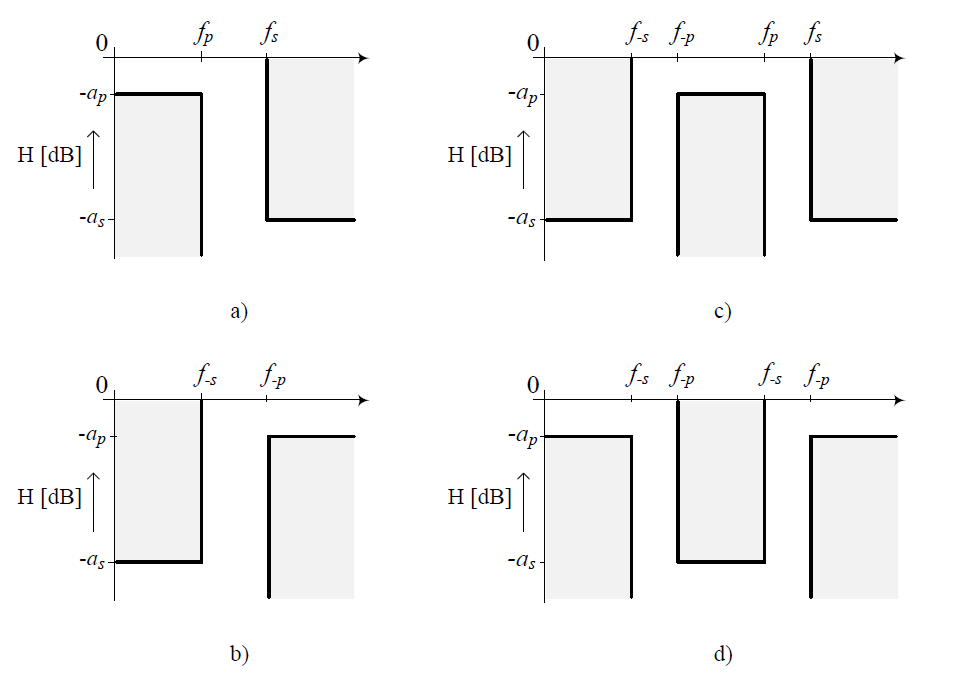
\includegraphics[scale=0.55]{tolerancnischemata.png}
\caption[Toleranční schéma dolní propusti (DP), horní propusti (HP), pásmové propusti (PP) a pásmové zádrže]{Toleranční schéma pro a) dolní propust (DP), b) horní propust (HP), c) pásmovou propust (PP) a d) pásmovou zádrž (PZ)\cite{7}}
\end{figure}
\noindent Dolní propust nepropouští na výstup vstupní signál nad frekvencí $f_s$, signál v propustném pásmu zůstává beze změny nebo zesílený. Základní pasivní dvojbranné zapojení je ke vstupu sériově zapojený rezistor a k této větvi paralelně kapacitor. Tento RC člen - integrační článek se zvyšující se frekvencí snižuje svou vstupní impedanci. Přenosová funkce v nekonečnu je nulová. \\
Obecná přenosová funkce filtru typu dolní propust n-tého řádu je podle Vedrala a Svatoše~\cite{19}
\begin{equation}
H(p) = \frac{H_0}{\prod_{i=1}^{\frac{n}{2}} (1 + a_i p + b_i p^2)} \label{r:FTR},
\end{equation}
kde $n$ je řád filtru a $p = j\omega/omega_0$, $\omega_0$ je mezní kruhový kmitočet filtru, při kterém klesne jeho přenos o 3 dB vzhledem ke stejnosměrnému přenosu.\\
\\
Dolní propust druhého řádu má přenos v nekonečnu nulový $H_{\infty} = 0$. \\
Horní propust nepropouští signály o nízkých frekvencích. Nejjednodušší zapojení je RC člen - derivační článek, kde kapacitor je zapojen sériově se zdrojem a k této větvi paralelně rezistor. Pro toto zapojení reaktance kapacitoru se zvyšující se frekvencí klesá. Přenosová funkce ideálního derivačního článku je v nule nulová. \\
Obecná přenosová funkce filtru typu horní propust n-tého řádu je podle Vedrala a Svatoše~\cite{19}
\begin{equation}
H(p) = \frac{H_{\infty}}{\prod_{i=1}^{\frac{n}{2}} (1 + \frac{a_i}{p} + \frac{b_i}{p^2})} \label{r:FTR2},
\end{equation}
kde $n$ je řád filtru a $H_{\infty}$ přenos filtru pro $\omega \gg \omega_0$.\\
\\
\noindent Pásmová propust propouští pásmo určené dvěma kmitočty. Pasivní pásmové propusti nedosahují účinnosti větší než 1. Jsou složeny z integračního článku (RC - dolní propust) a derivačního článku (CR - horní propust) zapojených v sérii, viz obrázek \ref{s:BPBS}. Ideální pásmová propust má přenos v nule i nekonečnu nulový. \\
\begin{figure}[h]
\centering
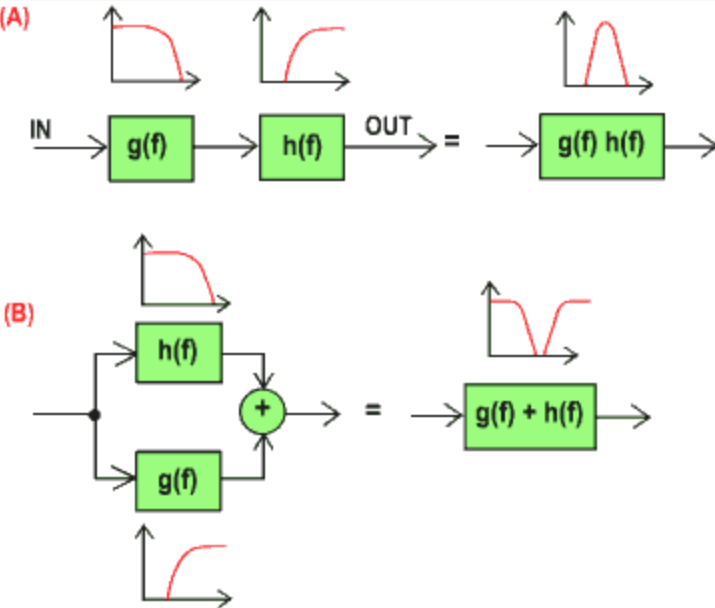
\includegraphics[scale=0.6]{bpbs.png}
\caption[A) Násobení přenosů - pásmová propust, B) Sčítání přenosů - pásmová zádrž]{A) Násobení přenosů - pásmová propust, B) Sčítání přenosů - pásmová zádrž \cite{8} \label{s:BPBS}}
\end{figure}
\noindent Pásmová propust má přenos v nule i nekonečnu nulový $H_{0} = H_{\infty} = 0$. Její přenosová funkce je~\cite{12}
\begin{equation}
H(p) = \frac{H_{B} \frac{\omega _0}{Q} (p) }{p^2 + \frac{\omega _0}{Q}(p) + \omega _0 ^2}.
\end{equation}
Pásmová zádrž nepropouští kmitočty pásma definovaného dvěma kmitočty. Pasivní zapojení je složeno ze dvou rezistorů a kapacitorů. Má vždy ztrátový přenos. Ideální pásmová zádrž má přenosovou funkci v nule stejnou jako v nekonečnu. Lze ji složit sečtením přenosů horní a dolní propusti, viz obrázek \ref{s:BPBS}. Její přenosová funkce je~\cite{12}
\begin{equation}
H(p) = \frac{H_{0} (p^2 + \omega_0^2)}{p^2 + \frac{\omega _0}{Q}(p) + \omega _0 ^2}.
\end{equation}
\subsection{Aproximace}
Podle rozložení nul a pólů jmenovatele rozlišujeme různé aproximace. Úlohou aproximace je nalézt k zadanému tolerančními schématu přenosovou funkci. Koeficienty filtru $a_i, b_i$ (viz rovnice \ref{r:FTR}, \ref{r:FTR2}) určují zesílení v propustném pásmu. Činitel jakosti udává míru ztrát v rezonančním obvodu a je definován jako $Q = \sqrt{b_i}/a_i$. Čím větší $Q$ je obdrženo, tím spíš bude filtr nestabilní. U cívek je nositelem ztrát zejména odpor vodiče, kterým jsou navinuty. U kondenzátorů určují Q hlavně dielektrické ztráty použitého dielektrika (Suchánek \cite{6}).\\
Pro následující charakteristiky také zadefinujeme fázový posuv a skupinové zpoždění. Fázový posuv je podle Vedrala a Svatoše \cite{19} výstupního napětí filtru vzhledem k jeho vstupnímu napětí je úměrný řádu filtru a kmitočtu.
\begin{equation}
\phi _n(\omega) \approx arctg(n \frac{\omega}{\omega _0}) \label{s:ROV}
\end{equation}
V rovnici \ref{s:ROV} je n řád filtru a $\omega _0$ mezní kruhový kmitočet.\\
Skupinové zpoždění filtru je definované poměrem změny fáze ke změně úhlového kmitočtu a je přímo úměrné řádu filtru a kmitočtu.\\
\begin{equation}
T _{DPn}(\omega) = \frac{d\phi}{d\omega} = - \frac{n}{\omega _0},
\end{equation}
\noindent kde n je řád filtru.\\
\begin{figure}[h]
\centering
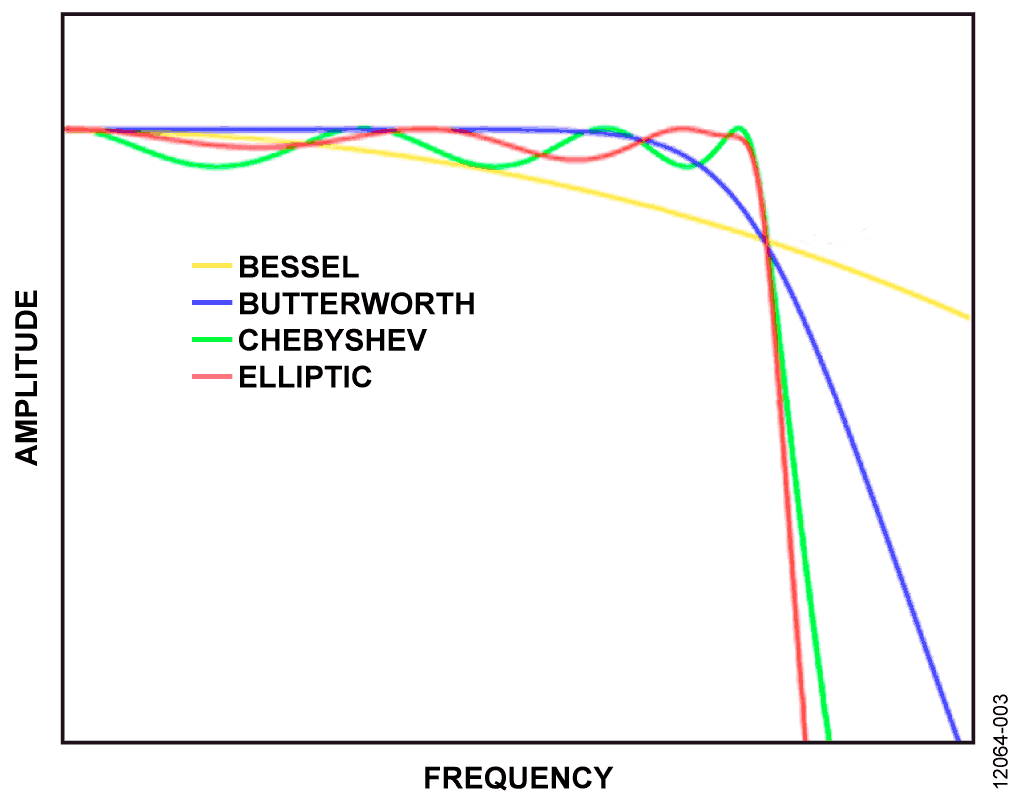
\includegraphics[scale=0.3]{LGA98.png}
\caption[Typy aproximací (DP)]{Typy aproximací (DP)\cite{9}}
\end{figure}
\subsection{Butterworthova aproximace}
Podle Kašpera \cite{7} má Butterworthova aproximace maximálně plochou amplitudovou charakteristiku v propustném pásmu. Má monotónní průběh v propustném i nepropustném pásmu. Frekvenční charakteristika má sklon daný počtem pólů a pro její posouzení je užíváno skupinové zpoždění (derivace fáze podle frekvence). Pro Butterworthovu aproximaci je skupinové zpoždění nezvlněné v propustném pásmu. Přechodová charakteristika má mírný překmit, zvyšující se s řádem filtru. Zesílení $G(\omega)$ je kmitočtově závislé a odpovídá absolutní hodnotě přenosové funkce $H(p)$. Platí
\begin{equation}
|H(p)| = \frac{1}{\sqrt{1 + \epsilon ^2 \frac{\omega}{\omega _0}^{2n}}},
\end{equation}
kde $\epsilon$ je poměrné zvlnění kmitočtové charakteristiky v propustném pásmu (faktor zvlnění), $n$ je řád filtru a $\omega _0$ mezní kruhový kmitočet (nastává při útlumu 3 dB). Pro $\omega _0 = 1$ je faktor zvlnění $\epsilon = 1$. 
\subsection{Čebyševova aproximace}
Podle Kašpera \cite{7} má Čebyševova aproximace strmější pokles útlumové charakteristiky v přechodovém pásmu, což vede na nižší stupeň přenosové funkce a užití nižšího řádu filtru než u Butterworthovy aproximace. Zato má ale zvlněnou frekvenční charakteristiku v propustném pásmu. Oproti Butterworthově aproximaci má tedy vlastnosti z hlediska průběhu fázové charakteristiky a skupinového zpoždění horší (Martinek, Boreš, Hospodka \cite{10}).
\subsubsection{Typ I}
Vyjádření modulové charakteristiky pro tuto aproximaci je dáno jako
\begin{align}
G(\omega) = |H(p)| = \frac{1}{\sqrt{1 + \epsilon ^2 T_n ^2 \frac{\omega}{\omega _0}^{2n}}},
\end{align}
kde $T_n$ je Čebyševův polynom, $\epsilon$ je poměrné zvlnění, $n$ je řád filtru a $\omega _0$ mezní kruhový kmitočet. Čebyševův polynom je definován vztahem $2 \omega ^2 - 1$ pro $n = 2$. Obecně jsou to kořeny Čebyševových diferenciálních rovnic
\begin{align}
(1 - x^2)y" - xy' + n^2y &= 0,\\
(1 - x^2)y" - 3xy' + n(n+2)y &= 0.
\end{align}
\subsubsection{Typ II}
Typ II je nazýván také jako inverzní Čebeševova aproximace. V praxi není příliš používaný, jelikož nemá tak rychlý pokles jako typ I a k jeho realizaci je třeba více prvků. Nemá zvlnění v propustném pásmu (monotónní průběh), zato v zádržném ano. Podle Kašpera \cite{7} je zesílení definováno jako
\begin{equation}
G(\omega, \omega _0) = \frac{1}{\sqrt{1 + \frac{1}{\epsilon ^2 T_n ^2 \frac{\omega _0}{\omega}^{2n}}}},
\end{equation}
kde $T_n$ je Čebyševův polynom, $\epsilon$ je poměrné zvlnění, $n$ je řád filtru a $\omega _0$ mezní kruhový kmitočet.
\subsection{Besselova aproximace}
Besselova aproximace se podle Kašpera \cite{7} používá v telekomunikační technice v případech, kdy je požadováno zachování tvaru signálu. Amplitudová charakteristika v nepropustném pásmu je velmi plochá. Koeficienty polynomu jsou zvoleny tak, aby fázová charakteristika v pásmu okolo kritické frekvence byla maximálně lineární. Nevýhodou je poměrně malá strmost modulové charakteristiky. Ta je pro Besselovu aproximaci dána vztahem
\begin{equation}
|H(p)| = \frac{\Theta _n(0)}{\Theta _n(\frac{p}{\omega _0})},
\end{equation}
kde $\Phi _n$ je Besselův polynom a $\omega _0$ mezní kruhový kmitočet. Besselův polynom je definován součtem řady
\begin{equation}
\Theta _n (x) = x^n y_n (\frac{1}{x}) = \sum_{k=0}^{n}\frac{(n+k)!}{(n-k)!k!}\frac{x^{n-k}}{2^k}.
\end{equation}
Pro filtr druhého řádu platí
\begin{equation}
G(\omega) = |H(p)| = \frac{3}{\sqrt{\omega ^4 + 3\omega ^2 + 9}}.
\end{equation}
\subsection{Cauerova (eliptická) aproximace}
\noindent Cauerova aproximace (eliptická) má podle Kašpera \cite{7} nejstrmější pokles, při jejím užití jsou voleny nižší řády filtru. Pokud se zvlnění v zádržném pásmu blíží nule, filtr se stává Čebyševovým (výše zmíněný - typ I). Opačně je tomu v propustném pásmu - přiblížením k nule se filtr stává inverzním Čebyševovým (typ II).  Pokud se obě hodnoty zvlnění blíží k nule, filtr se stává Butterworthovým. Kmitočtová charakteristika je dána vztahem
\begin{equation}
G(\omega) = |H(p)| = \frac{1}{\sqrt{1 + \epsilon ^2 R_n ^2(\zeta, \frac{\omega}{\omega _0})}},
\end{equation}
kde $\epsilon$ je faktor zvlnění, $R_n$ eliptická racionální funkce n-tého řádu, $\zeta$ selektivní faktor a $\omega _0$ mezní kruhový kmitočet. Pokud pro selektivní faktor platí $\zeta \rightarrow \infty$, filtr se stává Čebyševovým (typ I).\\
\\
Protože se, podobně jako u Čebyševovy aproximace, liší odvození pro liché a sudé stupně, jsou pro ně různé postupy. Pro lichý stupeň existuje pouze jedna varianta, pro sudý tři varianty (A, B, C), které se liší průběhem aproximační funkce, viz Martinek, Boreš, Hospodka \cite{10}.
\subsubsection{Cauerova (eliptická) aproximace typu A}
Má stejný počet pólů a nul aproximující funkce. Je realizována jako LC filtr (sekce \ref{s:LC}) pouze s vázanými induktory.
\subsubsection{Cauerova (eliptická) aproximace typu B}
Jedná se o posun útlumového pólu z konečného kmitočtu k nekonečnu, tedy dále od propustného pásma. Tato úprava vede ke snížení strmosti přechodu od propustného k nepropustnému pásmu. Je to obdoba postupu u inverzní Čebyševovy aproximace. Tento typ je nejčastěji používaný.
\subsubsection{Cauerova (eliptická) aproximace typu C}
Vhodnou transformací, která vede na nulovou hodnotu přenosu v nulovém kmitočtu, získáme navíc proti variantám A, B i shodné zakončovací odpory v případě LC realizace (sekce \ref{s:LC}). Je to obdoba postupu u Čebyševovy aproximace.
\subsection{Srovnání typů aproximací}
Podle Martinka \cite{10} není z hlediska zápisu přenosové funkce rozdíl mezi Butterworthovou a Čebyševovou aproximací, přestože jedna má v propustném pásmu hladký a druhá zvlněný průběh. Přenosová funkce má v čitateli konstantu a ve jmenovateli polynom (odtud společné označení polynomiální aproximace).\\
Oproti tomu volba průběhu v nepropustném pásmu tvar přenosové funkce mění. Pokud je průběh monotónní (Butterworthova, Čebyševova aproximace), jedná se o podíl konstanty a polynomu. Je-li průběh v nepropustném pásmu zvlněný, tvoří přenosovou funkci podíl dvou polynomů. Pro běžné aproximace (Cauerova, inverzní Čebyševova) je v čitateli sudý polynom ve tvaru $\prod _{i} (p^2 + \omega_i^2)$.\\
Volbou kombinace hladkého a zvlěného průběhu v propustném a nepropustném pásmu získáme různé vlastnosti.\\
\newpage
 \begin{table}[h]
 \caption[Přehled aproximací podle tvaru aproximační funkce v propustném i nepropustném pásmu]{\label{tab:Přehled aproximací podle tvaru aproximační funkce v propustném i nepropustném pásmu}Přehled aproximací podle tvaru aproximační funkce v propustném i nepropustném pásmu \cite{10}}
  \end{table}
\begin{center}
\begin{table}[h]
\centering
  \begin{tabular}{ | c | c | c | }
    \hline
    Propustné pásmo & Nepropustné pásmo & Příklad aproximace \\ \hline
    hladká & hladká & Butterworthova \\ \hline
    zvlněná & hladká & Čebyševova \\ \hline
    hladká & zvlněná & inverzní Čebyševova \\ \hline
    zvlněná & zvlněná & Cauerova \\ \hline
  \end{tabular}
   \end{table}
   \end{center}